
%% bare_conf.tex
%% V1.3
%% 2007/01/11
%% by Michael Shell
%% See:
%% http://www.michaelshell.org/
%% for current contact information.
%%
%% This is a skeleton file demonstrating the use of IEEEtran.cls
%% (requires IEEEtran.cls version 1.7 or later) with an IEEE conference paper.
%%
%% Support sites:
%% http://www.michaelshell.org/tex/ieeetran/
%% http://www.ctan.org/tex-archive/macros/latex/contrib/IEEEtran/
%% and
%% http://www.ieee.org/

%%*************************************************************************
%% Legal Notice:
%% This code is offered as-is without any warranty either expressed or
%% implied; without even the implied warranty of MERCHANTABILITY or
%% FITNESS FOR A PARTICULAR PURPOSE! 
%% User assumes all risk.
%% In no event shall IEEE or any contributor to this code be liable for
%% any damages or losses, including, but not limited to, incidental,
%% consequential, or any other damages, resulting from the use or misuse
%% of any information contained here.
%%
%% All comments are the opinions of their respective authors and are not
%% necessarily endorsed by the IEEE.
%%
%% This work is distributed under the LaTeX Project Public License (LPPL)
%% ( http://www.latex-project.org/ ) version 1.3, and may be freely used,
%% distributed and modified. A copy of the LPPL, version 1.3, is included
%% in the base LaTeX documentation of all distributions of LaTeX released
%% 2003/12/01 or later.
%% Retain all contribution notices and credits.
%% ** Modified files should be clearly indicated as such, including  **
%% ** renaming them and changing author support contact information. **
%%
%% File list of work: IEEEtran.cls, IEEEtran_HOWTO.pdf, bare_adv.tex,
%%                    bare_conf.tex, bare_jrnl.tex, bare_jrnl_compsoc.tex
%%*************************************************************************

% *** Authors should verify (and, if needed, correct) their LaTeX system  ***
% *** with the testflow diagnostic prior to trusting their LaTeX platform ***
% *** with production work. IEEE's font choices can trigger bugs that do  ***
% *** not appear when using other class files.                            ***
% The testflow support page is at:
% http://www.michaelshell.org/tex/testflow/



% Note that the a4paper option is mainly intended so that authors in
% countries using A4 can easily print to A4 and see how their papers will
% look in print - the typesetting of the document will not typically be
% affected with changes in paper size (but the bottom and side margins will).
% Use the testflow package mentioned above to verify correct handling of
% both paper sizes by the user's LaTeX system.
%
% Also note that the "draftcls" or "draftclsnofoot", not "draft", option
% should be used if it is desired that the figures are to be displayed in
% draft mode.
%
\documentclass[conference]{IEEEtran}
% Add the compsoc option for Computer Society conferences.
%
% If IEEEtran.cls has not been installed into the LaTeX system files,
% manually specify the path to it like:
% \documentclass[conference]{../sty/IEEEtran}





% Some very useful LaTeX packages include:
% (uncomment the ones you want to load)


% *** MISC UTILITY PACKAGES ***
%
%\usepackage{ifpdf}
% Heiko Oberdiek's ifpdf.sty is very useful if you need conditional
% compilation based on whether the output is pdf or dvi.
% usage:
% \ifpdf
%   % pdf code
% \else
%   % dvi code
% \fi
% The latest version of ifpdf.sty can be obtained from:
% http://www.ctan.org/tex-archive/macros/latex/contrib/oberdiek/
% Also, note that IEEEtran.cls V1.7 and later provides a builtin
% \ifCLASSINFOpdf conditional that works the same way.
% When switching from latex to pdflatex and vice-versa, the compiler may
% have to be run twice to clear warning/error messages.



\usepackage{booktabs,tabularx}


% *** CITATION PACKAGES ***
%
\usepackage{cite}
% cite.sty was written by Donald Arseneau
% V1.6 and later of IEEEtran pre-defines the format of the cite.sty package
% \cite{} output to follow that of IEEE. Loading the cite package will
% result in citation numbers being automatically sorted and properly
% "compressed/ranged". e.g., [1], [9], [2], [7], [5], [6] without using
% cite.sty will become [1], [2], [5]--[7], [9] using cite.sty. cite.sty's
% \cite will automatically add leading space, if needed. Use cite.sty's
% noadjust option (cite.sty V3.8 and later) if you want to turn this off.
% cite.sty is already installed on most LaTeX systems. Be sure and use
% version 4.0 (2003-05-27) and later if using hyperref.sty. cite.sty does
% not currently provide for hyperlinked citations.
% The latest version can be obtained at:
% http://www.ctan.org/tex-archive/macros/latex/contrib/cite/
% The documentation is contained in the cite.sty file itself.






% *** GRAPHICS RELATED PACKAGES ***
%
\ifCLASSINFOpdf
   \usepackage[pdftex]{graphicx}
  % declare the path(s) where your graphic files are
  % \graphicspath{{../pdf/}{../jpeg/}}
  % and their extensions so you won't have to specify these with
  % every instance of \includegraphics
  % \DeclareGraphicsExtensions{.pdf,.jpeg,.png}
\else
  % or other class option (dvipsone, dvipdf, if not using dvips). graphicx
  % will default to the driver specified in the system graphics.cfg if no
  % driver is specified.
  % \usepackage[dvips]{graphicx}
  % declare the path(s) where your graphic files are
  % \graphicspath{{../eps/}}
  % and their extensions so you won't have to specify these with
  % every instance of \includegraphics
  % \DeclareGraphicsExtensions{.eps}
\fi
% graphicx was written by David Carlisle and Sebastian Rahtz. It is
% required if you want graphics, photos, etc. graphicx.sty is already
% installed on most LaTeX systems. The latest version and documentation can
% be obtained at: 
% http://www.ctan.org/tex-archive/macros/latex/required/graphics/
% Another good source of documentation is "Using Imported Graphics in
% LaTeX2e" by Keith Reckdahl which can be found as epslatex.ps or
% epslatex.pdf at: http://www.ctan.org/tex-archive/info/
%
% latex, and pdflatex in dvi mode, support graphics in encapsulated
% postscript (.eps) format. pdflatex in pdf mode supports graphics
% in .pdf, .jpeg, .png and .mps (metapost) formats. Users should ensure
% that all non-photo figures use a vector format (.eps, .pdf, .mps) and
% not a bitmapped formats (.jpeg, .png). IEEE frowns on bitmapped formats
% which can result in "jaggedy"/blurry rendering of lines and letters as
% well as large increases in file sizes.
%
% You can find documentation about the pdfTeX application at:
% http://www.tug.org/applications/pdftex





% *** MATH PACKAGES ***
%
%\usepackage[cmex10]{amsmath}
% A popular package from the American Mathematical Society that provides
% many useful and powerful commands for dealing with mathematics. If using
% it, be sure to load this package with the cmex10 option to ensure that
% only type 1 fonts will utilized at all point sizes. Without this option,
% it is possible that some math symbols, particularly those within
% footnotes, will be rendered in bitmap form which will result in a
% document that can not be IEEE Xplore compliant!
%
% Also, note that the amsmath package sets \interdisplaylinepenalty to 10000
% thus preventing page breaks from occurring within multiline equations. Use:
%\interdisplaylinepenalty=2500
% after loading amsmath to restore such page breaks as IEEEtran.cls normally
% does. amsmath.sty is already installed on most LaTeX systems. The latest
% version and documentation can be obtained at:
% http://www.ctan.org/tex-archive/macros/latex/required/amslatex/math/





% *** SPECIALIZED LIST PACKAGES ***
%
%\usepackage{algorithmic}
% algorithmic.sty was written by Peter Williams and Rogerio Brito.
% This package provides an algorithmic environment fo describing algorithms.
% You can use the algorithmic environment in-text or within a figure
% environment to provide for a floating algorithm. Do NOT use the algorithm
% floating environment provided by algorithm.sty (by the same authors) or
% algorithm2e.sty (by Christophe Fiorio) as IEEE does not use dedicated
% algorithm float types and packages that provide these will not provide
% correct IEEE style captions. The latest version and documentation of
% algorithmic.sty can be obtained at:
% http://www.ctan.org/tex-archive/macros/latex/contrib/algorithms/
% There is also a support site at:
% http://algorithms.berlios.de/index.html
% Also of interest may be the (relatively newer and more customizable)
% algorithmicx.sty package by Szasz Janos:
% http://www.ctan.org/tex-archive/macros/latex/contrib/algorithmicx/




% *** ALIGNMENT PACKAGES ***
%
%\usepackage{array}
% Frank Mittelbach's and David Carlisle's array.sty patches and improves
% the standard LaTeX2e array and tabular environments to provide better
% appearance and additional user controls. As the default LaTeX2e table
% generation code is lacking to the point of almost being broken with
% respect to the quality of the end results, all users are strongly
% advised to use an enhanced (at the very least that provided by array.sty)
% set of table tools. array.sty is already installed on most systems. The
% latest version and documentation can be obtained at:
% http://www.ctan.org/tex-archive/macros/latex/required/tools/


%\usepackage{mdwmath}
%\usepackage{mdwtab}
% Also highly recommended is Mark Wooding's extremely powerful MDW tools,
% especially mdwmath.sty and mdwtab.sty which are used to format equations
% and tables, respectively. The MDWtools set is already installed on most
% LaTeX systems. The lastest version and documentation is available at:
% http://www.ctan.org/tex-archive/macros/latex/contrib/mdwtools/


% IEEEtran contains the IEEEeqnarray family of commands that can be used to
% generate multiline equations as well as matrices, tables, etc., of high
% quality.


%\usepackage{eqparbox}
% Also of notable interest is Scott Pakin's eqparbox package for creating
% (automatically sized) equal width boxes - aka "natural width parboxes".
% Available at:
% http://www.ctan.org/tex-archive/macros/latex/contrib/eqparbox/





% *** SUBFIGURE PACKAGES ***
%\usepackage[tight,footnotesize]{subfigure}
% subfigure.sty was written by Steven Douglas Cochran. This package makes it
% easy to put subfigures in your figures. e.g., "Figure 1a and 1b". For IEEE
% work, it is a good idea to load it with the tight package option to reduce
% the amount of white space around the subfigures. subfigure.sty is already
% installed on most LaTeX systems. The latest version and documentation can
% be obtained at:
% http://www.ctan.org/tex-archive/obsolete/macros/latex/contrib/subfigure/
% subfigure.sty has been superceeded by subfig.sty.



%\usepackage[caption=false]{caption}
%\usepackage[font=footnotesize]{subfig}
% subfig.sty, also written by Steven Douglas Cochran, is the modern
% replacement for subfigure.sty. However, subfig.sty requires and
% automatically loads Axel Sommerfeldt's caption.sty which will override
% IEEEtran.cls handling of captions and this will result in nonIEEE style
% figure/table captions. To prevent this problem, be sure and preload
% caption.sty with its "caption=false" package option. This is will preserve
% IEEEtran.cls handing of captions. Version 1.3 (2005/06/28) and later 
% (recommended due to many improvements over 1.2) of subfig.sty supports
% the caption=false option directly:
%\usepackage[caption=false,font=footnotesize]{subfig}
%
% The latest version and documentation can be obtained at:
% http://www.ctan.org/tex-archive/macros/latex/contrib/subfig/
% The latest version and documentation of caption.sty can be obtained at:
% http://www.ctan.org/tex-archive/macros/latex/contrib/caption/




% *** FLOAT PACKAGES ***
%
%\usepackage{fixltx2e}
% fixltx2e, the successor to the earlier fix2col.sty, was written by
% Frank Mittelbach and David Carlisle. This package corrects a few problems
% in the LaTeX2e kernel, the most notable of which is that in current
% LaTeX2e releases, the ordering of single and double column floats is not
% guaranteed to be preserved. Thus, an unpatched LaTeX2e can allow a
% single column figure to be placed prior to an earlier double column
% figure. The latest version and documentation can be found at:
% http://www.ctan.org/tex-archive/macros/latex/base/



%\usepackage{stfloats}
% stfloats.sty was written by Sigitas Tolusis. This package gives LaTeX2e
% the ability to do double column floats at the bottom of the page as well
% as the top. (e.g., "\begin{figure*}[!b]" is not normally possible in
% LaTeX2e). It also provides a command:
%\fnbelowfloat
% to enable the placement of footnotes below bottom floats (the standard
% LaTeX2e kernel puts them above bottom floats). This is an invasive package
% which rewrites many portions of the LaTeX2e float routines. It may not work
% with other packages that modify the LaTeX2e float routines. The latest
% version and documentation can be obtained at:
% http://www.ctan.org/tex-archive/macros/latex/contrib/sttools/
% Documentation is contained in the stfloats.sty comments as well as in the
% presfull.pdf file. Do not use the stfloats baselinefloat ability as IEEE
% does not allow \baselineskip to stretch. Authors submitting work to the
% IEEE should note that IEEE rarely uses double column equations and
% that authors should try to avoid such use. Do not be tempted to use the
% cuted.sty or midfloat.sty packages (also by Sigitas Tolusis) as IEEE does
% not format its papers in such ways.





% *** PDF, URL AND HYPERLINK PACKAGES ***
%
%\usepackage{url}
% url.sty was written by Donald Arseneau. It provides better support for
% handling and breaking URLs. url.sty is already installed on most LaTeX
% systems. The latest version can be obtained at:
% http://www.ctan.org/tex-archive/macros/latex/contrib/misc/
% Read the url.sty source comments for usage information. Basically,
% \url{my_url_here}.





% *** Do not adjust lengths that control margins, column widths, etc. ***
% *** Do not use packages that alter fonts (such as pslatex).         ***
% There should be no need to do such things with IEEEtran.cls V1.6 and later.
% (Unless specifically asked to do so by the journal or conference you plan
% to submit to, of course. )


% correct bad hyphenation here
\hyphenation{op-tical net-works semi-conduc-tor}


\begin{document}
%
% paper title
% can use linebreaks \\ within to get better formatting as desired
\title{Final Report Group 1}


% author names and affiliations
% use a multiple column layout for up to three different
% affiliations
%\author{\IEEEauthorblockN{Michael Shell}
%\IEEEauthorblockA{School of Electrical and\\Computer Engineering\\
%Georgia Institute of Technology\\
%Atlanta, Georgia 30332--0250\\
%Email: http://www.michaelshell.org/contact.html}
%\and
%\IEEEauthorblockN{Homer Simpson}
%\IEEEauthorblockA{Twentieth Century Fox\\
%Springfield, USA\\
%Email: homer@thesimpsons.com}
%\and
%\IEEEauthorblockN{James Kirk\\ and Montgomery Scott}
%\IEEEauthorblockA{Starfleet Academy\\
%San Francisco, California 96678-2391\\
%Telephone: (800) 555--1212\\
%Fax: (888) 555--1212}}

\author{Helton Chen 260410774  \and Claus Choy 260454385 \and Andrew Jesson 260196340 \and Meng Yin Tao 260480207}

% conference papers do not typically use \thanks and this command
% is locked out in conference mode. If really needed, such as for
% the acknowledgment of grants, issue a \IEEEoverridecommandlockouts
% after \documentclass

% for over three affiliations, or if they all won't fit within the width
% of the page, use this alternative format:
% 
%\author{\IEEEauthorblockN{Michael Shell\IEEEauthorrefmark{1},
%Homer Simpson\IEEEauthorrefmark{2},
%James Kirk\IEEEauthorrefmark{3}, 
%Montgomery Scott\IEEEauthorrefmark{3} and
%Eldon Tyrell\IEEEauthorrefmark{4}}
%\IEEEauthorblockA{\IEEEauthorrefmark{1}School of Electrical and Computer Engineering\\
%Georgia Institute of Technology,
%Atlanta, Georgia 30332--0250\\ Email: see http://www.michaelshell.org/contact.html}
%\IEEEauthorblockA{\IEEEauthorrefmark{2}Twentieth Century Fox, Springfield, USA\\
%Email: homer@thesimpsons.com}
%\IEEEauthorblockA{\IEEEauthorrefmark{3}Starfleet Academy, San Francisco, California 96678-2391\\
%Telephone: (800) 555--1212, Fax: (888) 555--1212}
%\IEEEauthorblockA{\IEEEauthorrefmark{4}Tyrell Inc., 123 Replicant Street, Los Angeles, California 90210--4321}}




% use for special paper notices
%\IEEEspecialpapernotice{(Invited Paper)}




% make the title area
\maketitle


\begin{abstract}
%\boldmath
The project implements a 5-stage pipelined processor and an assembler. The assembler turns the MIPS assembly code into 32-bit binary machine code instructions. The instructions propagate through the pipeline. Hazards are detected along the pipeline and dependent data are forwarded when possible.
\end{abstract}
% IEEEtran.cls defaults to using nonbold math in the Abstract.
% This preserves the distinction between vectors and scalars. However,
% if the conference you are submitting to favors bold math in the abstract,
% then you can use LaTeX's standard command \boldmath at the very start
% of the abstract to achieve this. Many IEEE journals/conferences frown on
% math in the abstract anyway.

% no keywords




% For peer review papers, you can put extra information on the cover
% page as needed:
% \ifCLASSOPTIONpeerreview
% \begin{center} \bfseries EDICS Category: 3-BBND \end{center}
% \fi
%
% For peerreview papers, this IEEEtran command inserts a page break and
% creates the second title. It will be ignored for other modes.
\IEEEpeerreviewmaketitle



\section{Problem Statement}

The processor implemented in this project translates MIPS assembly code into binary machine code. The instructions are executed using a 5-stage pipeline as shown in Figure \ref{pipelineBD} \cite{compOrg}. Control signals (in green), data lines (in blue) and register information (in yellow) propagate through the pipeline. Stall signals (in red) are used to prevent instructions (in purple) from entering the pipeline when hazards are detected.

\begin{figure}[!h]
\centering
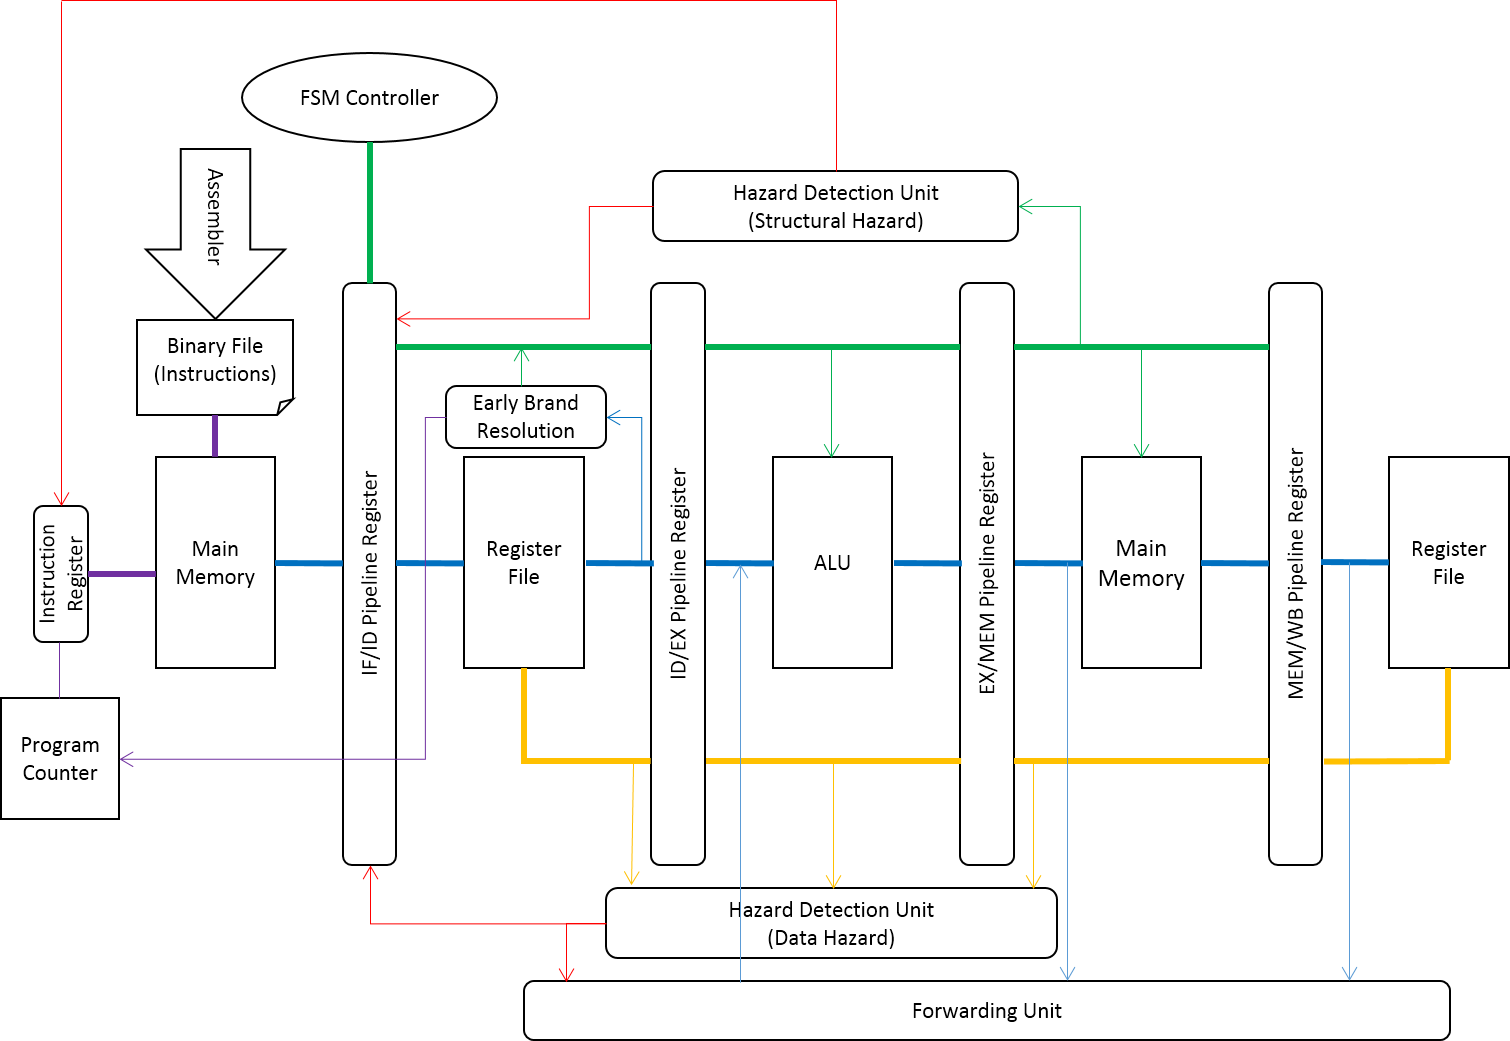
\includegraphics[width=2.5in]{Figures/pipeline}
\caption{Pipeline Processor Block Diagram}
\label{pipelineBD}
\end{figure}


\section{Components}

The system consists of two components: an assembler and a processor. The assembler translates the MIPS assembly code into binary instructions. The instructions are stored in the main memory along with the data. The processor accesses the main memory to fetch instructions, load data and store data. The processor is pipelined into five stages and uses hazard detection, a forwarding unit and early branch detection to reduce stalls.

\subsection{Assembler}

The assembler functions by first parsing the assembly code into a structured instruction table and then converting each row of the table into binary machine language. We have implemented the assembler in MATLAB.

\subsubsection{Parsing Assembly Language}
To parse the assembly language the input file is first opened and read line by line. For each line comments are removed and labels are checked for. If the line is still not empty the mnemonic of the instruction and arguments are parsed and stored. After this first iteration the assembler then searches for labels in the argument fields and calculates their offset to the label position. The resulting instruction table for fib.asm is shown in Table \ref{instructTable}. Aside from the arguments and names of each instruction, an array is stored identifying the basic block that the argument belongs to. Inner blocks are stored after Arg 3 and more general blocks are stored proceeding from left to right. 

\begin{table}[h]
\caption{Instruction table result of parsing fib.asm}
\label{instructTable}
\begin{tabular}{@{}llllllll@{}}
\toprule
Mnemonic & Type & Arg 1 & Arg 2 & Arg 3 & Block 1 & ... & Block N \\ \midrule
addi     & I    & \$10  & \$0   & 4     &         &     &         \\
addi     & I    & \$1   & \$0   & 1     &         &     &         \\
addi     & I    & \$2   & \$0   & 1     &         &     &         \\
addi     & I    & \$11  & \$0   & 2000  &         &     &         \\
addi     & I    & \$15  & \$0   & 4     &         &     &         \\
addi     & I    & \$3   & \$2   & 0     & loop    &     &         \\
add      & R    & \$2   & \$2   & \$1   & loop    &     &         \\
addi     & I    & \$1   & \$3   & 0     & loop    &     &         \\
mult     & R    & \$10  & \$15  &       & loop    &     &         \\
mflo     & R    & \$12  &       &       & loop    &     &         \\
add      & R    & \$13  & \$11  & \$12  & loop    &     &         \\
sw       & I    & \$2   & \$13  & 0     & loop    &     &         \\
addi     & I    & \$10  & \$10  & -1    & loop    &     &         \\
bne      & I    & \$10  & \$0   & -9    & loop    &     &         \\
beq      & I    & \$11  & \$11  & -1    &         &     &         \\ \bottomrule
\end{tabular}
\end{table}

\begin{figure}[!h]
\centering
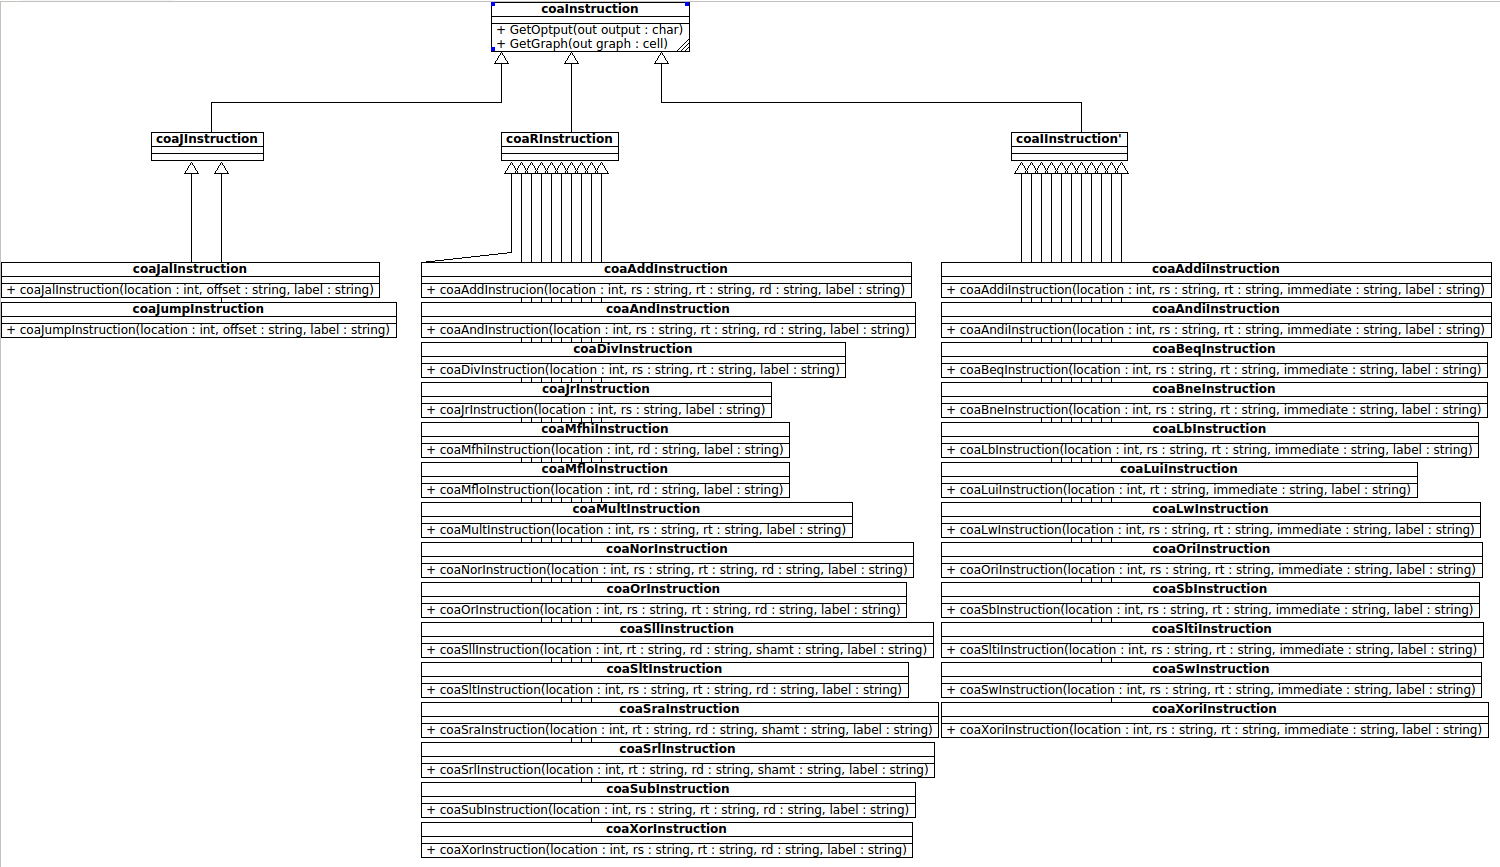
\includegraphics[width=2.5in]{Figures/coaAssemblerUML}
\caption{Class Hierarchy of Assembler Instruction Objects}
\label{classDiagram}
\end{figure}

\subsubsection{Converting Instruction Table to Binary Machine Language}
For this procedure we take an object oriented approach. This design decision was made to support easy extension of instructions not included in the specification. The class hierarchy of the instruction API is shown in Figure \ref{classDiagram}. The public class constructors take the form of coa<mnemonic>Instruction(args) and return an Instruction object, I. The args for each type of instruction are taken from the above described instruction table. The public I.GetOutput() method returns the line of binary machine language corresponding to the type of instruction and arguments passed. The public I.GetGraph() method returns a structured array of the position of the instruction within the program, the register it writes to, the registers it reads from, and minimum and maximum indices of the basic block it belongs to. This method has been designed to facilitate instruction rescheduling. Table \ref{depGraph} represents the graph that would correspond to fib.asm after the initializing a static rescheduling routine with the graphs from each instruction. The routine would then maximize the distance between the true data dependencies with constraints determined by the minimum and maximum positions, along with the anti and output dependencies.

\begin{table}[h]
\caption{First Iteration Dependencies Graph for Fib.asm}
\label{depGraph}
\begin{tabularx}{\columnwidth}{@{}lcccccccc@{}}
\toprule
Pos. & Write & Read 1 & Read 2 & Min Pos. & Max Pos. & True & Anti \\ \midrule
1 & 10 & 0 &  & 1 & 5 &  &  \\
2 & 1 & 0 &  & 1 & 5 &  &  \\
3 & 2 & 0 &  & 1 & 5 &  &  \\
4 & 11 & 0 &  & 1 & 5 &  &  \\
5 & 15 & 0 &  & 1 & 5 &  &  \\
6 & 3 & 2 &  & 6 & 13 & 3 &  \\
7 & 2 & 2 & 1 & 6 & 13 & 3 & 6  \\
8 & 1 & 3 &  & 6 & 13 & 6 &  \\
9 &  & 10 & 15 & 6 & 12 & 1,5 &   \\
10 & 12 &  &  & 7 & 13 &   & 9\\
11 & 13 & 11 & 12 & 6 & 13 & 4,10 &  \\ 
12 &  & 13 & 2 & 6 & 13 & 11,7 &  \\
13 & 10 & 10 &  & 6 & 13 & 1 &  9\\
14 &  & 10 & 0 & 14 & 14 & 13 &  \\
15 &  & 11 & 11 & 15 & 15 &  &  \\ \bottomrule
\end{tabularx}
\end{table}

\subsection{Instruction Fetch (IF) Stage}

The first stage of the pipeline consists of fetching an instruction from memory and updating the program counter (PC). By convention, instructions are stored sequentially and the first instruction starts at memory address 0x00. Every instruction is 32 bits long and memory is address by byte; therefore, instructions are separated by a 4 memory address offset.

\subsubsection{PC} 
The PC is programmed to increment by 0x04 at every clock cycle and used as a pointer to the next instruction . When a control flow instruction is detected, such as a branch or a jump, the target address is computed. A select signal is set high to take the target address and the PC is updated to use the new address for its next computation.

\subsection{Instruction Decode (ID) Stage}

Once the instruction is fetched from memory, it is decoded in the ID stage, where the OPCODE is sent to the pipeline controller. Depending on the current OPCODE and the last state, the pipeline controller will issue a series of control signals.  Depending on the type of MIPS instruction (R-type, I-type or J-type), the register file puts the corresponding data onto the register data line. To reduce stalling after a branch instruction, we implemented an early branch resolution unit. When a branch instruction is detected during the ID stage, the PC counter will first be instructed to update its value to the target address, then the IF/ID pipeline register will be warned that a branch instruction was detected, and finally the last instruction fetched will be flushed. The decoded instruction information and data are passed to the next stage through the ID/EX pipeline register.

\subsubsection{Pipeline Controller}
The pipeline controller is the most crucial component in the processor as it turns the OPCODE into control signals that oversees the execution of the pipeline. All control signals are updated during a single clock cycle and then fed to the IF/ID pipeline register. Control signals propagate through the pipeline and may be changed if a hazard is detected. 

\subsubsection{Register File}
This processor implementation uses 32-bit data registers. The register file stores the register values and is accessed depending on the instruction type. The first register (R0) is hardwired to 0x00. The register file reads its inputs on every rising clock edge and updates the corresponding registers. On the falling edge, the register file outputs the data requested. Therefore, during a single clock cycle, data can be written to and read from the register file. This implementation avoids stalling the pipeline when two instructions (one read and one write) need to access the registers.

\subsubsection{Early Branch Resolution Unit}
Branch hazards may cause the pipeline to fetch the wrong instruction when a branch prediction is wrong. In the current implementation, branches are predicted as not taken and the instruction stored immediately after the branch instruction is fetched while the branch instruction is in the ID stage. As the branch instruction propagates down the pipeline, more instructions are fetched until the branch is resolved. To avoid fetching extra instructions whose execution depends on the branch condition, an early branch resolution is implemented. It uses a comparator and resolves the branch condition in the IF stage. By doing so, it saves one clock cycle in the case when the branch prediction is wrong (branch is taken) and does not affect performance when the branch prediction is correct

\subsection{Execution (EX) Stage}

After the instruction is decoded, the operands are written to their respective data lines. The arithmetic logic unit (ALU) can now perform computation when needed. The inputs of the ALU depend both on the type of instruction and also when data is forwarded and are selected accordingly. The result of the ALU is passed on to the next stage through the EX/MEM pipeline register.

\subsubsection{ALU}
All computations are performed by the ALU. The ALU takes two 32-bit inputs and returns a 32-bit result.  The selection of input is managed by the pipeline controller and the forwarding unit. With the exception of MULT and DIV instructions, the result of the ALU computation is available after a single clock cycle. MULT and DIV instructions are expected to be followed by MFLO or MFHI instructions. 

\subsection{Memory Access (MEM) Stage}

Other than fetching an instruction, memory can be access only during a LOAD or STORE instruction. When an instruction arrives at this stage, the control signals will be used to determine if memory access is needed. The data loaded from the memory, is passed on to the next stage through the MEM/WB pipeline register. 

\subsubsection{Main Memory}
The main memory module used here was provided by the course TA. Unlike the register file, data cannot be written to and read from the main memory at the same time. This causes the pipeline to stall (disable data fetching) when a LOAD or a STORE instruction in its MEM stage. Due to the slow access time, main memory requires several clock cycles before returning the requested information.

\subsection{Write-Back (WB) Stage}

The final stage of the pipeline updates the register file with the computed value or the data loaded from memory. When an instruction arrives at this stage, the control signals will be used to determine if register access is needed. As previously mentioned, data can be written to and read from the register file in the same clock cycle, so no stall will be introduced­.

\subsection{Pipeline}

In order for the pipeline to function properly, the information of each stage is stored in the pipeline registers. With the intermediate values stored, it becomes possible to implement additional components to reduce the stall time between instructions such as, hazard detection and data forwarding.

\subsubsection{Pipeline Registers}
Registers are essential to the functioning of the pipeline. A pipeline register couples each stage and stores the information of an instruction. For instance, when an instruction moves from the ID stage to the EX stage, its control signals, data and register information are written to a pipeline register. These values kept in the register until the next clock cycle, where the instruction exits the EX stage. This register sits between the ID and the EX stage, therefore is called the ID/EX pipeline register. There are a total of five pipeline registers in this implementation: IF, IF/ID, ID/EX, EX/MEM and MEM/WB pipeline registers and so there are five instructions in the pipeline when the pipeline is fully loaded without stalls. All registers hold their values for one clock cycle and are updated at every rising edge of the clock. 

\subsubsection{Hazard Detection Unit}
As mentioned earlier, data cannot be written to or read from memory at the same time. This represents a structural hazard that requires the pipeline to stall until memory access is completed. A structural hazard detection unit is used to verify the control lines in the EX stage. If the instruction in the EX stage need to access memory (either read or write) in the next cycle, the structural hazard detection unit will issue a stall signal to disable instruction fetch at the next clock cycle. 

Data dependencies can also affect the performance of the processor in the case of a read-after-write (RAW) dependency. A data hazard detection unit is used to compare the input of one instruction against the output of the previous two instructions. When the instruction in the EX stage requires the ALU output of the instruction one cycle ahead of it, then a EX-to-EX forwarding is required. When the instruction in the EX stage requires the ALU output or the memory output of an instruction two cycles ahead of it, then a MEM-to-EX forwarding is required.

For both structural hazard detection unit and data hazard detection unit, all instructions following the instruction causing the stall are paused and only resume execution once the hazard is resolved.

Branch dependencies are not explicitly handled in the implementation. The early branch resolution unit is the only component that will reduce stall by one clock cycle  in the case of a wrong branch prediction as explained earlier.

\subsubsection{Forwarding Unit}
When data hazards are detected, the forwarding unit is signaled to forward data to the input of the ALU in the EX stage. Depending on the type of forwarding, the appropriate input is selected for the ALU.  A EX-to-EX forwarding will feed the ALU output directly back to its input. A MEM-to-EX forwarding will feed the output from the memory back to the input of the ALU. The forwarding unit avoids waiting for data to be written back to register before it becomes available to the following instructions. The forwarding unit also forwards to the early branch resolution unit, where the target address can be resolved earlier.

\subsection{Optimization}

\subsubsection{Branch Predictor}
A simple branch predictor can be implemented to predict branch not taken. It will reduce the number of wrong predictions in the case of looping. This branch predictor will be added early in the pipeline to update PC to the target address before knowing the outcome of the branch instruction. More complex branch predictors can also be used.

\subsubsection{Split Level-1 Cache}
A main cause for stalling is the long memory access time. To reduce waiting time, caches can be implemented. A split cache would be best because it would allow instruction fetching at the same time of a LOAD or STORE instruction accessing memory.

\subsubsection{Instruction Rescheduling}
Optimization could also be done by the assembler. A better assembler could detect independent instructions and insert them between dependent instructions that require extra clock cycles between them. The assembler could also detect loops and perform loop unrolling to allow more rescheduling possibilities.

\subsubsection{Branch Delay Slot}
nstead of using branch prediction, the branch delay slot can be populated with an instruction which will not affect the branch instruction. Since in the current implementation the instruction following the branch instruction is fetched regardless of the branch resolution, it could be replaced by an instruction that was originally before the branch instruction. This rescheduling of instructions must be done by the assembler. The assembler must make sure that the instruction in the branch delay slot will not affect the branch instruction outcome. 

\section{System Evaluation}

The pipelined system was successfully implemented for our project. Here we show relevant example outputs that show specific processor functions.

In Figure \ref{pc4} we can see that the program counter successfully increments by 4 on the next rising edge of clock signal which displays that it is functioning properly.

\begin{figure}[!h]
\centering
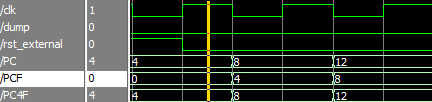
\includegraphics[width=2.5in]{Figures/PC_increment}
\caption{Incrementing the program counter.}
\label{pc4}
\end{figure}

Figure \ref{aluAdd} shows that the inputs to the ALU are returning the correct results at its output. Here we show three instructions being executed, the first instruction is an addi, followed by an add and then another addi. Our processor correctly chooses the right signal using the decoded instruction.

\begin{figure}[!h]
\centering
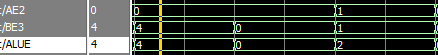
\includegraphics[width=2.5in]{Figures/add}
\caption{Testing the ALU with an add operation.}
\label{aluAdd}
\end{figure}

Figure \ref{stall} shows that when a store instruction is executed, our processor stalls for one clock cycle and so when a stall occurs the PC and INSTR are present for a total of two clock cycles. We can see this on the rising edge of the clock when the program counter is at 56. The representation of the Instruction is in decimals in this case to save space.

\begin{figure}[!h]
\centering
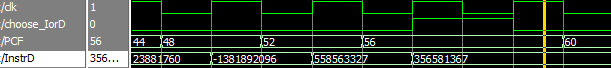
\includegraphics[width=2.5in]{Figures/stall}
\caption{Demonstrating stalling on load and store operations.}
\label{stall}
\end{figure}

In Figure \ref{pipeProp}, we can see the propagation of the RegWrite control signal through the pipeline. The last letter in the signal name specifies in which section of the pipeline the signal is in. Therefore, we can see the same signal propagating from the decode stage all the way to the write back stage. We can also see that the signal is delayed by one clock cycle per stage which is what is expected in a pipelined processor.

\begin{figure}[!h]
\centering
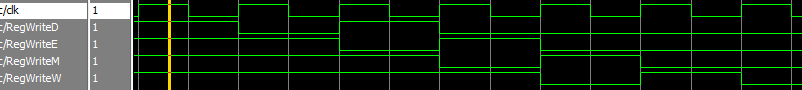
\includegraphics[width=2.5in]{Figures/pipeline_prop}
\caption{Demonstrating propagation of control signals through the pipeline}
\label{pipeProp}
\end{figure}

In Figure \ref{instDecEx} we show one of our larger tests to determine correct instruction decode and execution. We used the instruction: addi \$10, \$0, 4 where the value in \$0 is 0. The instruction is correctly decoded from our assembler and in our processor the corresponding ALU instruction is fed into the ALU; which is an add instruction. Rs and Rt are also selected correctly with Rt as the destination register and Rs as one of the sources. We can also see that the Immediate value is 4, which is what was required. Following the decode stage we can see that the values being fed into the ALU are again correct and happen one cycle later. We can also verify that the output of the ALU is correct as 0 + 4 = 4 as desired.

\begin{figure}[!h]
\centering
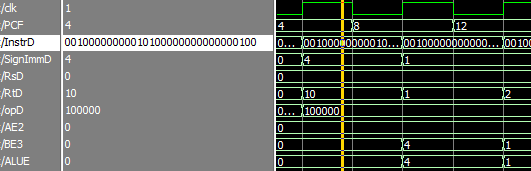
\includegraphics[width=2.5in]{Figures/instr_decode_execute}
\caption{Demonstrating instruction decode and execution.}
\label{instDecEx}
\end{figure}

\section{Recommendation}

As we look back on how the project was approached, the main challenge was to get the first implementation to work. If we had the opportunity to start the project all over again, we would like to perform functional tests on each individual components before assembling the entire processor. We have under-estimated the time needed to both assemble and test the processor. After combining all components in a single VHDL file, we had many errors preventing the program from simulating. It was hard to find out what might have caused each issue due to the complexity of the connections and the multiple number of components. For the second deliverable it was particularly hard to insert new components. Instead of modifying the first deliverable, we decided to restructure the entire processor. To avoid having to debug or modifying a large file, we think it would be preferable to have multiple small deliverables. We propose to breakdown the project into pipeline stages instead of changing a functional implementation into a pipeline. For instance, the first deliverable could consist of fetching and decoding the instruction. This deliverable will focus on on accessing the memory, interpreting the instruction code, and generating control signals. The second deliverable could be the execution which would aim at creating an execution stage that takes the right input and performs the correct operation depending on the control signals. The third deliverable could be the memory access and hazard detection. During this deliverable, we will detect hazards and stall the pipeline when needed. Finally, the last deliverable will consists of the write-back and forwarding. We think by building the project stage by stage, it would be easier to debug knowing that the previous stage is working properly.


% An example of a floating figure using the graphicx package.
% Note that \label must occur AFTER (or within) \caption.
% For figures, \caption should occur after the \includegraphics.
% Note that IEEEtran v1.7 and later has special internal code that
% is designed to preserve the operation of \label within \caption
% even when the captionsoff option is in effect. However, because
% of issues like this, it may be the safest practice to put all your
% \label just after \caption rather than within \caption{}.
%
% Reminder: the "draftcls" or "draftclsnofoot", not "draft", class
% option should be used if it is desired that the figures are to be
% displayed while in draft mode.
%
%\begin{figure}[!t]
%\centering
%\includegraphics[width=2.5in]{myfigure}
% where an .eps filename suffix will be assumed under latex, 
% and a .pdf suffix will be assumed for pdflatex; or what has been declared
% via \DeclareGraphicsExtensions.
%\caption{Simulation Results}
%\label{fig_sim}
%\end{figure}

% Note that IEEE typically puts floats only at the top, even when this
% results in a large percentage of a column being occupied by floats.


% An example of a double column floating figure using two subfigures.
% (The subfig.sty package must be loaded for this to work.)
% The subfigure \label commands are set within each subfloat command, the
% \label for the overall figure must come after \caption.
% \hfil must be used as a separator to get equal spacing.
% The subfigure.sty package works much the same way, except \subfigure is
% used instead of \subfloat.
%
%\begin{figure*}[!t]
%\centerline{\subfloat[Case I]\includegraphics[width=2.5in]{subfigcase1}%
%\label{fig_first_case}}
%\hfil
%\subfloat[Case II]{\includegraphics[width=2.5in]{subfigcase2}%
%\label{fig_second_case}}}
%\caption{Simulation results}
%\label{fig_sim}
%\end{figure*}
%
% Note that often IEEE papers with subfigures do not employ subfigure
% captions (using the optional argument to \subfloat), but instead will
% reference/describe all of them (a), (b), etc., within the main caption.


% An example of a floating table. Note that, for IEEE style tables, the 
% \caption command should come BEFORE the table. Table text will default to
% \footnotesize as IEEE normally uses this smaller font for tables.
% The \label must come after \caption as always.
%
%\begin{table}[!t]
%% increase table row spacing, adjust to taste
%\renewcommand{\arraystretch}{1.3}
% if using array.sty, it might be a good idea to tweak the value of
% \extrarowheight as needed to properly center the text within the cells
%\caption{An Example of a Table}
%\label{table_example}
%\centering
%% Some packages, such as MDW tools, offer better commands for making tables
%% than the plain LaTeX2e tabular which is used here.
%\begin{tabular}{|c||c|}
%\hline
%One & Two\\
%\hline
%Three & Four\\
%\hline
%\end{tabular}
%\end{table}


% Note that IEEE does not put floats in the very first column - or typically
% anywhere on the first page for that matter. Also, in-text middle ("here")
% positioning is not used. Most IEEE journals/conferences use top floats
% exclusively. Note that, LaTeX2e, unlike IEEE journals/conferences, places
% footnotes above bottom floats. This can be corrected via the \fnbelowfloat
% command of the stfloats package.


\begin{thebibliography}{1}

\bibitem{compOrg}
D.~Patterson and J.~ Hennessy, \emph{Computer Organization and Design}, 4th~ed.\hskip 1em plus
  0.5em minus 0.4em\relax Waltham, MA: Morgan Kaufmann, 2012.

\end{thebibliography}




% that's all folks
\end{document}


